\def\pgfsysdriver{pgfsys-dvipdfm.def}
\documentclass[aspectratio43]{beamer}
\usepackage{fontspec}
\setmainfont[Mapping=tex-text]{Arial}
\setsansfont[Mapping=tex-text]{Arial}
\setmonofont[Mapping=tex-text]{Arial}
\usepackage[russian]{babel}
\usetheme{default}
%\setbeameroption{show notes}
\usepackage{listings}
\usepackage{hyperref}
\usepackage{caption}
\usepackage{subcaption}
\usepackage{tabularx}
\usepackage{advdate}
\usepackage{pgfpages}
\usepackage{pifont}
%\renewcommand\tabularxcolumn[1]{m{#1}}   

\usepackage{adjustbox}
\usepackage{tabularx}

\usepackage{tikz}
\usetikzlibrary{automata,positioning,arrows.meta,calc,shapes.geometric}
\tikzset{>={Stealth[width=3mm,length=3mm]}}

%-------------------------------------------------------------------------------
\setbeamertemplate{navigation symbols}{}
\setbeamertemplate{itemize subitem}{\ding{226}}
%\setbeameroption{hide notes} % Only slides
\setbeameroption{show only notes} % Only notes
%\setbeameroption{show notes on second screen=right} % Both
\setbeamertemplate{note page}{\pagecolor{yellow!5}\vfill\insertnote\vfill}
\setbeamertemplate{headline}{%
\leavevmode%
    \hbox{%
        \begin{beamercolorbox}[wd=\paperwidth,ht=2.25ex,dp=1ex,center]{section in head/foot}%
            \usebeamerfont{section in head/foot}\insertsectionhead
        \end{beamercolorbox}%
    }
}
\makeatletter
\setbeamertemplate{footline}
{
    \leavevmode%
    \hbox{%
        \begin{beamercolorbox}[wd=.333333\paperwidth,ht=2.25ex,dp=1ex,center]{date in head/foot}%
            \usebeamerfont{author in head/foot}\insertshortauthor
        \end{beamercolorbox}%
        \begin{beamercolorbox}[wd=.333333\paperwidth,ht=2.25ex,dp=1ex,center]{date in head/foot}%
            \usebeamerfont{title in head/foot}\insertshorttitle
        \end{beamercolorbox}%
        \begin{beamercolorbox}[wd=.333333\paperwidth,ht=2.25ex,dp=1ex,right]{date in head/foot}%
            \usebeamerfont{date in head/foot}\insertshortdate{}\hspace*{2em}
            \insertframenumber{} / \inserttotalframenumber\hspace*{2ex} 
        \end{beamercolorbox}}%
        \vskip0pt%
    }
\makeatother

%-------------------------------------------------------------------------------
\title[]{Универсальный механизм первичного поиска повторов в тексте для пакета Duplicate Finder}
\author[Глазырин Антон]{
	Глазырин Антон Георгиевич\\[1ex]
 	{\small Научный руководитель: доц. каф. СП, к.ф-м.н. Луцив Д.\,В.\\[0.5ex]}
 	{\small Рецензент: ген. дир. ООО <<Ембокс>> Бондарев А.\,В.\\}
}
\institute[]{СПбГУ}
\date{\SetDate[06/06/2023]\today}

\begin{document}
	
%==============================================================================

\begin{frame}
\titlepage

\note{
	Добрый день, меня зовут Глазырин Антон, и тема моей работы --- универсальный механизм первичного поиска повторов в тексте для пакета Duplicate Finder.
}
\end{frame}

%==============================================================================

\begin{frame}\frametitle{Мотивация}
\begin{itemize}
	\item E. Juergens, J. Porubän: $\approx$10\% документации --- дублированные фрагменты
	\item Негативное влияние повторов:
	\begin{itemize}
		\item Раздувание объема
		\item Усложнение модификации
	\end{itemize}
	\item Управление повторами --- улучшение документации
\end{itemize}

\note{
	Несколько слов про повторы в документации. Существует ряд исследований, которые показывают, что в среднем достаточно значительная часть документации крупных проектов --- около 10\% --- представляет собой дублированные фрагменты. Хотя повторы в документации сами по себе не являются чем-то плохим, они могут приводить к некоторым негативным последствиям, таким как раздувание объема документации и усложнение внесения изменений, что затрудняет сопровождение. Кроме того, существуют различные методы по улучшению документации, основанные на управлении повторами.
}
\end{frame}

%==============================================================================

\begin{frame}\frametitle{Мотивация: Duplicate Finder}
	\begin{figure}
		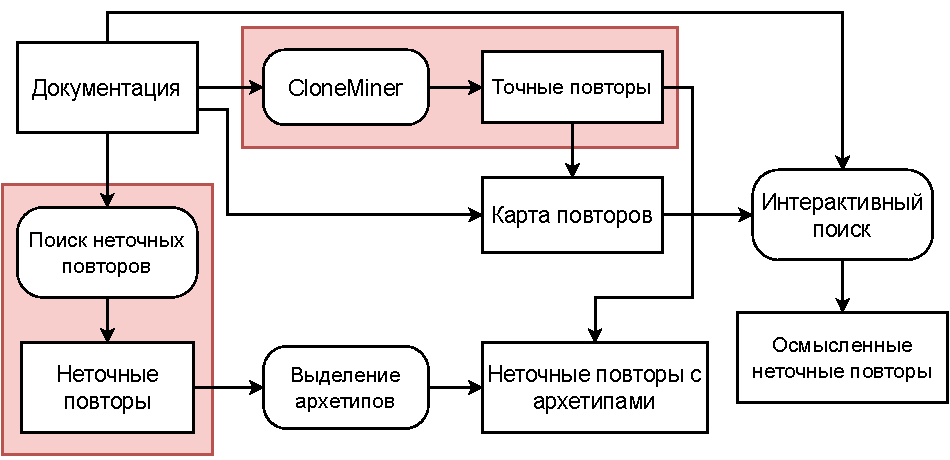
\includegraphics[scale=0.7]{../diploma/pictures/DuplicateFinder.pdf}
	\end{figure}
	
	\note{
		Один из таких методов лежит в основе пакета Duplicate Finder. Этот инструмент является университетской разработкой и предоставляет функционал для улучшения документации за счет поиска повторов. Из-за того, что данный проект разрабатывался и дополнялся в течение длительного промежутка времени многими разными людьми, у него появился ряд проблем с компонентами поиска. Дело в том, что в Duplicate Finder нет своего механизма поиска повторов: для этого используются набор внешних инструментов. Однако, эти инструменты написаны на разных языках, больше не поддерживаются, а самый важный из них --- CloneMiner --- является закрытой разработкой.
	}
\end{frame}

%==============================================================================

\begin{frame}\frametitle{Постановка задачи}
	Цель --- разработка унифицированной подсистемы поиска точных и неточных повторов для Duplicate Finder Toolkit.	
	
	\begin{itemize}
		\item Анализ предметной области
		\item Определение проблем поиска повторов в DuplicateFinder и требований к новому механизму
		\item Проектирование конвейера механизма поиска повторов
		\item Разработка алгоритмов точного и неточного поиска
		\item Реализация инструмента и его интеграция в DuplicateFinder
		\item Проведение тестирования разработанного инструмента
	\end{itemize}

	\note{
		Таким образом, целью данной работы является разработка унифицированной подсистемы поиска точных и неточных повторов для Duplicate Finder Toolkit. Для достижения данной цели были поставлены следующие задачи: ...
	}
\end{frame}

%==============================================================================

\begin{frame}\frametitle{Существующие решения}
	\begin{itemize}
		\item Поиск клонов в ПО:
		\begin{itemize}
			\item CCFinder
			\item CloneMiner
			\item Klocwork inSight
			\item cpdetector
		\end{itemize}
		\item Сравнение текстовых документов:
		\begin{itemize}
			\item Align
			\item TxtAlign
		\end{itemize} 
		\item Поиск по образцу: 
		\begin{itemize}
			\item Duplicate Defect Detection
			\item Apache Lucene
			\item FactorLCS
		\end{itemize}
	\end{itemize}

	\note{
		Поиск повторов очень широко распространен в различных сферах, и часто инструменты достаточно сильно заточны под свою конкретную задачу. Среди областей применения наиболее выделяются следующие. Это поиск клонов в исходном коде ПО: такие инструменты как CCFinder или CloneMiner, который как раз и используется в Duplicate Finder, сравнение текстовых документов: самый яркий пример --- это проверка на плагиат: такие инструменты как Align и TxtAlign, и поиск похожих вхождений по образцу: например, библиотека для поиска Apache Lucene.
	}
\end{frame}

%===============================================================================

\begin{frame}\frametitle{Определение требований}
	\begin{enumerate}
		\item Реализация на языке Python
		\item Открытая разработка
		\item Поиск точных и неточных повторов
		\item Универсальность процесса поиска
		\item Наличие API и CLI
		\item Возможность настройки
	\end{enumerate}

	\note{
		На основе анализа проблем поиска повторов в Duplicate Finder определены следующие требования к новому механизму: инструмент должен быть реализован на языке Python для максимальной совместимости с Duplicate Finder, быть открытой разработкой, и иметь возможности как точного так и неточного поиска повторов, сам процесс поиска должен быть универсальным, необходимо наличие API и CLI и должна быть возможность настройки параметров алгоритмов поиска.
	}
\end{frame}

%===============================================================================

\begin{frame}\frametitle{Конвейер поиска повторов}
	\begin{figure}
		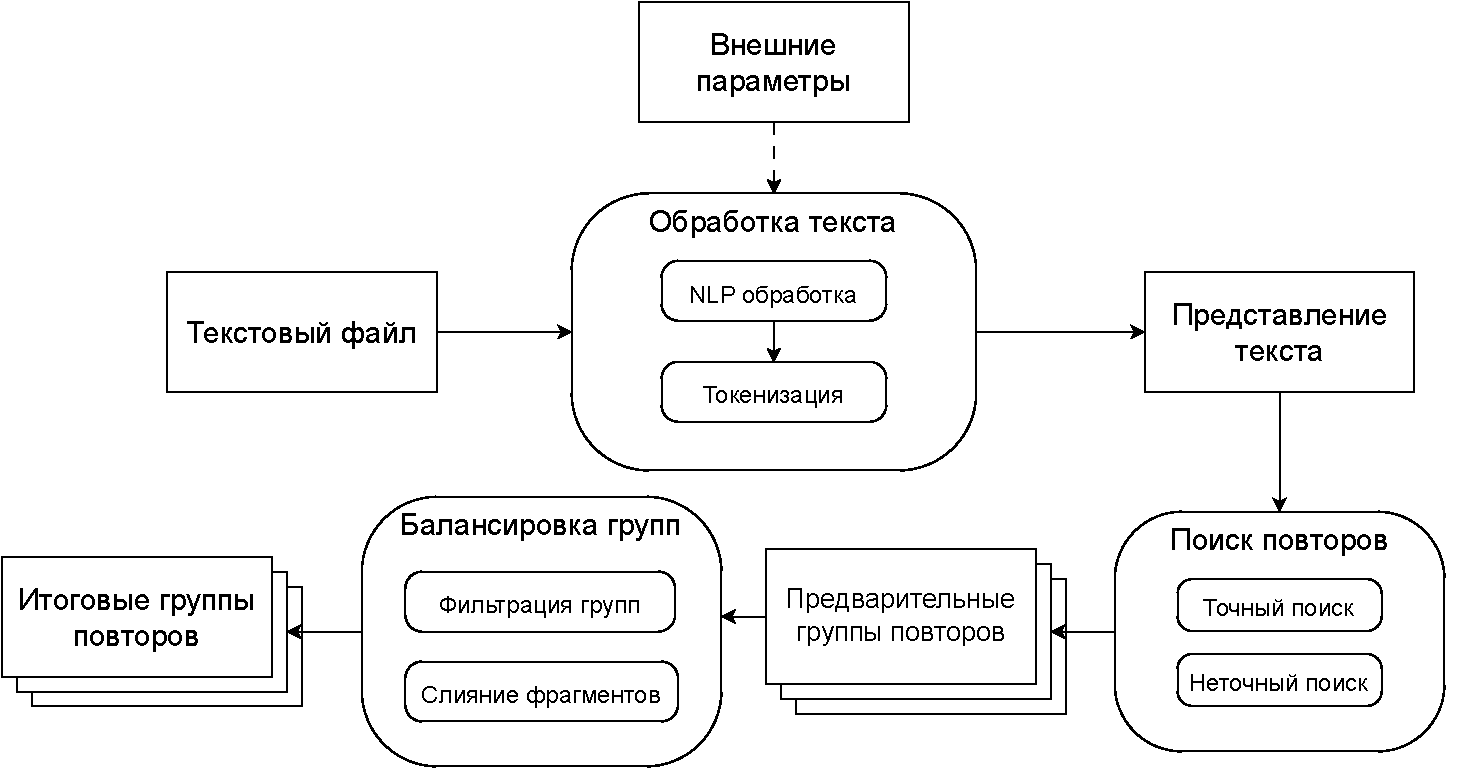
\includegraphics[scale=0.45]{../diploma/pictures/Pipeline.pdf}
	\end{figure}

	\note{
		На данном слайде представлена схема разработанного конвейера поиска повторов. Он включает в себя 3 основных этапа: предобработку текста для улучшения качества поиска, непосредственно применение алгоритмов поиска повторов, и затем балансировку полученных групп с целью улучшить качество результатов. Далее рассмотрим каждый этап подробнее.
	}
\end{frame}


%===============================================================================

\begin{frame}\frametitle{Предобработка текста}
	Методы NLP:
	\begin{itemize}
		\item Фильтрация спецсимволов
		\item Удаление стоп слов
		\item Лемматизация
		\item Стемминг
	\end{itemize}

	\note{
		Первым шагом является предобработка, которая выполняет 2 задачи: во-первых --- преобразование текста в удобный для дальнейшей работы вид, во-вторых --- применение ряда методов для облегчения работы алгоритмов поиска. Конкретно --- это подходы, широко используемые в NLP --- обработке естественного языка. Они включают в себя устранение шума --- фильтрацию спецсимволов и удаление стоп слов, а также приведение слов к наиболее унифицированной форме при помощи лемматизаци и стемминга. Кроме того текст токенизируется, и в дальнейшем представляется в виде набора токенов.
	}
\end{frame}


%===============================================================================

\begin{frame}\frametitle{Поиск точных повторов}

	\begin{figure}
		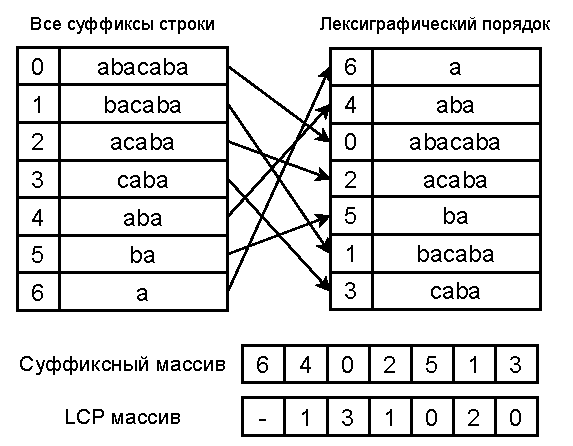
\includegraphics[scale=0.9]{../diploma/pictures/SA-LCP.pdf}
	\end{figure}

	\note{
		Далее рассмотрим алгоритмы поиска повторов. Всего были разработаны 3 алгоритма на основе компонент из Duplicate Finder: один для точного поиска и два для неточного. Алгоритм точного поиска основывается на построении суффиксного массива, который представляет собой последовательность суффиксов строки, упорядоченных в лексиграфическом порядке. Суть алгоритма заключается в том, что если в тексте содержатся два одинаковых фрагмента, то суффиксы, начинающиеся с этих фрагментов, будут соседями с суффиксном массиве, таким образом анализируя его можно находить и объединять повторы в группы.
	}
\end{frame}

%===============================================================================

\begin{frame}\frametitle{Поиск неточных повторов I}
	Расстояние Левенштейна:
	
	\begin{figure}
		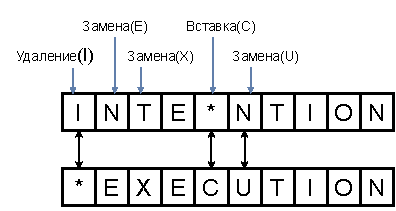
\includegraphics[scale=1.2]{../diploma/pictures/Edit-dist.pdf}
	\end{figure}

	\note{
		Первый алгоритм неточного поиска основан на вычисление расстояния Левинштейна между фрагментами --- количество операций удаления, замены и вставки нужное, чтобы превратить одну строку в другую. Если расстояние достаточно маленькое --- значит фрагменты похожи и являются неточными повторами. Однако вычисление расстояния Левинштейна достаточно трудоемкий процесс, и не имеет смысла проводить этот расчет для сильно различающихся фрагментов.
	}
\end{frame}

%===============================================================================

\begin{frame}\frametitle{Поиск неточных повторов I}
	SimHash:
	
	\begin{figure}
		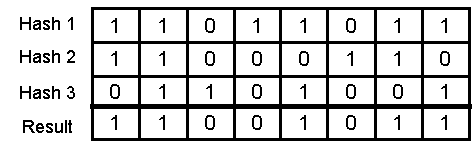
\includegraphics[scale=1.2]{../diploma/pictures/Hash.pdf}
	\end{figure}
	
	\note{
		 Для грубой оценки схожести можно использовать хеширование, в частности --- подход SimHash, который позволяет определить хеш коллекции на основе хешей ее составных частей, и затем использовать его для сравнения. Таким образом, фрагменты, имеющие много общих токенов, будут иметь схожие хеши. Суть алгоритма заключается в разбиение текста на фрагменты и попарного их сравнения при помощи этих двух подходов, с последующим объединением найденный пар в группы.
	}
\end{frame}

%===============================================================================

\begin{frame}\frametitle{Поиск неточных повторов II}
	Множества N-грамм:
	\begin{figure}
		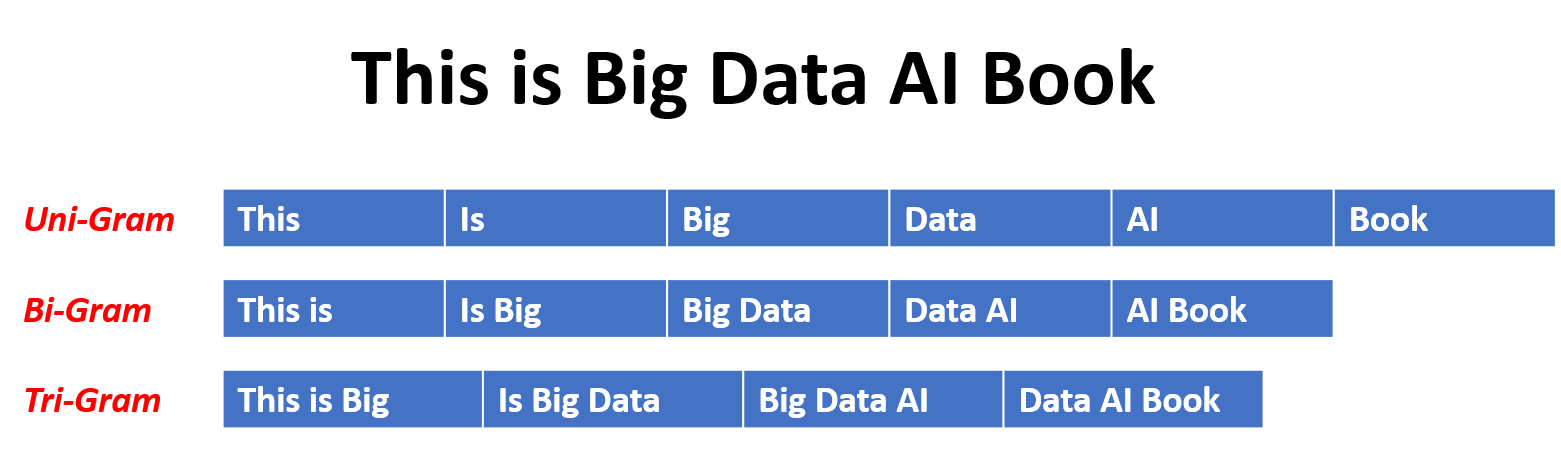
\includegraphics[scale=0.27]{../diploma/pictures/ngram.png}
	\end{figure}

	\note{
		Второй алгоритм неточного поиска основан на еще одном распространенном подходе для оценки схожести текстов --- построении множества N-грам. Имея два фрагмента можно построить их множества и вычислить пересечение, и чем ближе мощность полученного множества к исходному, тем больше эти фрагменты имеют одинаковых текстовых участков. Суть алгоритма заключается в разбиении текста на предложения и объединение их в группы повторов на основе вычисления пересечений их множеств N-грам.
	}
\end{frame}

%===============================================================================

\begin{frame}\frametitle{Балансировка групп повторов}
	\begin{itemize}
		\item Фильтрация незначимых групп
		\item Слияние фрагментов
	\end{itemize}

	\begin{figure}
		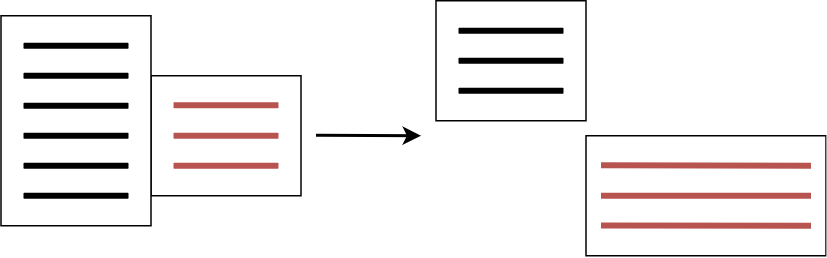
\includegraphics[scale=0.3]{../diploma/pictures/Balance3.png}
	\end{figure}

	\note{
		Последним этапом конвейера является балансировка групп повторов. Он включает в себя удаление незначимых групп --- которые содержат меньше 2 фрагментов, и слияние фрагментов --- если есть группы, все фрагменты которых находятся в исходном тексте рядом с фрагментами другой группы, можно перераспределить эти фрагменты между группами и объединить их, что повышает значимость результатов поиска.
	}
\end{frame}

%===============================================================================

\begin{frame}\frametitle{Архитектура}
	\begin{figure}
		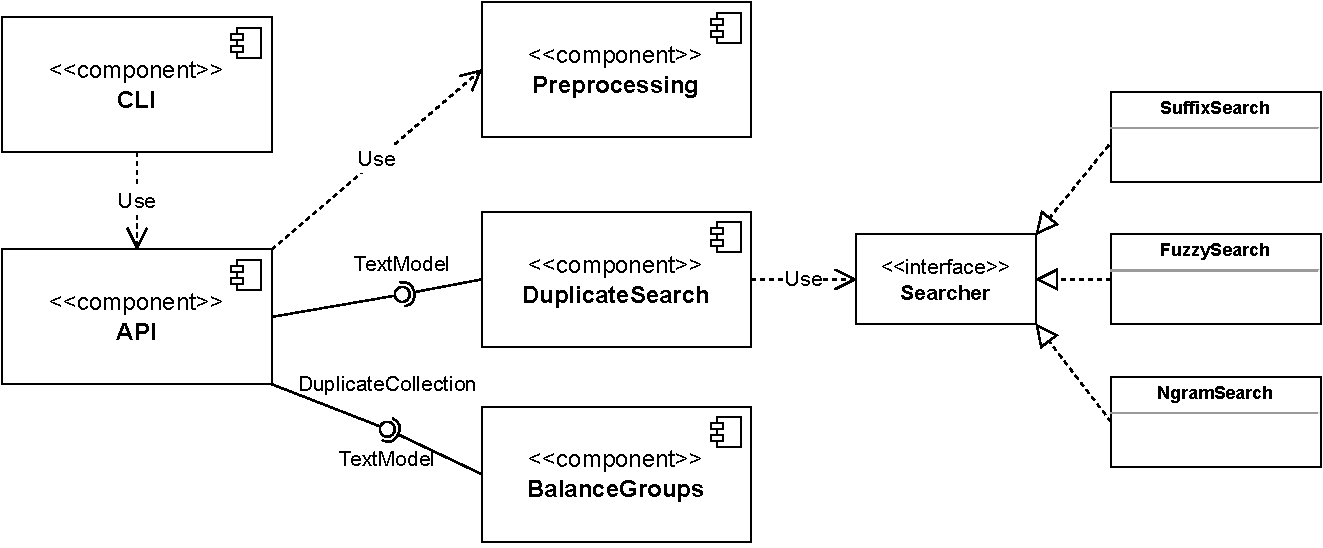
\includegraphics[scale=0.51]{../diploma/pictures/Architecture.pdf}
	\end{figure}

	\note{
		На данном слайде приведена архитектура реализованного инструмента. За каждый этап конвейера отвечает своя компонента, что позволят легко влиять на процесс поиска и добавлять новые алгоритмы.
	}
\end{frame}

%===============================================================================

\begin{frame}\frametitle{Тестирование: неточный поиск}
	
	\begin{figure}[h!]
		\centering
		\begin{minipage}{0.9\textwidth}
\begin{adjustbox}{center}
\begin{tabular}{|l||m{0.15\textwidth}|m{0.15\textwidth}|m{0.15\textwidth}|m{0.2\textwidth}|}
	\hline
	Документ & Группы повторов & Средний размер группы & Средняя длина повтора & Покрытие документа \\
	\hline
	\hline
	GIMP Manual & 574 & 2,65 & 13,64 & 15\% \\
	\hline
	PostgreSQL Manual & 464 & 2,66 & 17,17 & 25\% \\
	\hline
	Subversion book & 282 & 2,27 & 18,93 & 10\% \\
	\hline
	Zend Framework guide & 522 & 2,32 & 22,96 & 16\% \\
	\hline
	Blender Manual & 1393 & 2,48 & 14,22 & 16\% \\
	\hline
	Python Requests & 23 & 2,26 & 20,16 & 28\% \\
	\hline
\end{tabular}
\end{adjustbox}
\end{minipage}
	\end{figure}
	
	\note{
		Для тестирования были выбраны документации ряда различных крупных проектов. Для каждого документа был выполнен поиск точных и неточных повторов. Результаты приведены на слайде: неточный поиск...
	}
\end{frame}

%===============================================================================

\begin{frame}\frametitle{Тестирование: точный поиск}
	\begin{figure}[h!]
		\centering
		\begin{minipage}{0.9\textwidth}
\begin{adjustbox}{center}
\begin{tabular}{|l||c|c|c|c|}
	\hline
	& GIMP & PostgreSQL & Subversion & Zend Framework \\
	\hline
	\hline
	Токены & 132554 & 72728 & 110270 & 164035 \\
	\hline
	Группы повторов & 400 & 289 & 218  & 557 \\
	\hline
	Средний размер группы & 2.57 & 2.30 & 2.17 & 2.44 \\
	\hline
	Средняя длина повтора & 14.59 & 16.31 & 17.27 & 16.58 \\
	\hline
	Покрытие документа & ~11\% & ~14\% & ~7\% & ~13\% \\
	\hline
	
\end{tabular}
\end{adjustbox}
\end{minipage}
	\end{figure}

	\note{
		... и точный поиск. Как видно по результатам, инструмент хорошо находит как точные, так и неточные повторы. Кроме того, на практике подтверждается теоретические ожидания: примерно 10\% документа составляют дублированные участки. Исключением является Python Requests, которая представляет собой API-документацию и содержит много однообразного кода и описаний. Это также отражает идею, что в некоторых случаях повторы в документации неизбежны и выполняют определенную задачу.
	}
\end{frame}

%===============================================================================

\begin{frame}\frametitle{Тестирование: сравнение с CloneMiner}
	\begin{figure}[h!]
		\centering
		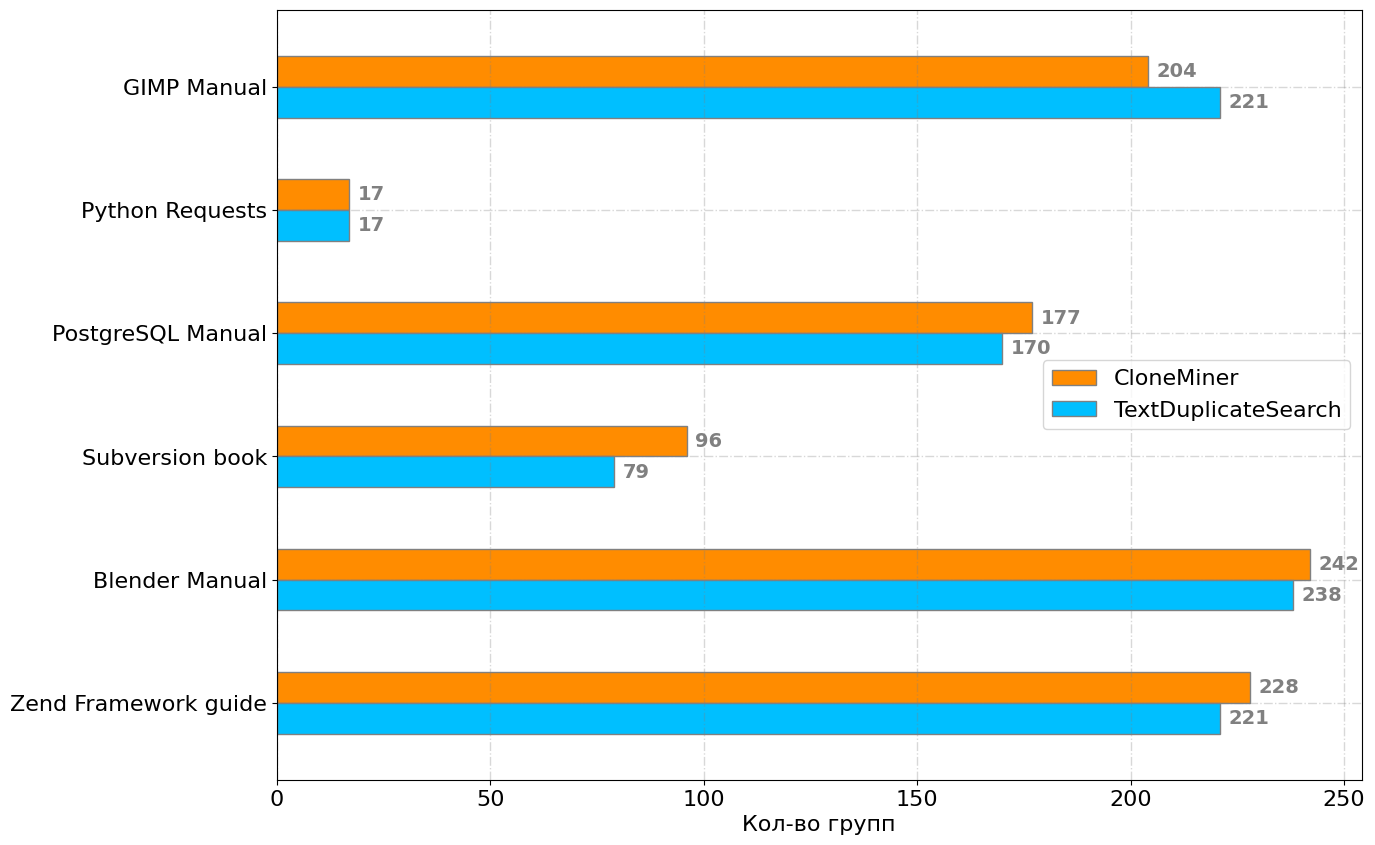
\includegraphics[scale=0.32]{../diploma/pictures/Comp1.png}
	\end{figure}
	
	\note{
		Также была проведена интеграция реализованного инструмента в DuplicateFinder и его сравнение с основным используемым там инструментом CloneMiner. На данном графике показано сколько групп повторов было найдено для документов при использовании каждого инструмента отельно от Duplicate Finder'a.
	}
\end{frame}

%===============================================================================

\begin{frame}\frametitle{Тестирование: сравнение с CloneMiner}
	\begin{figure}[h!]
		\centering
		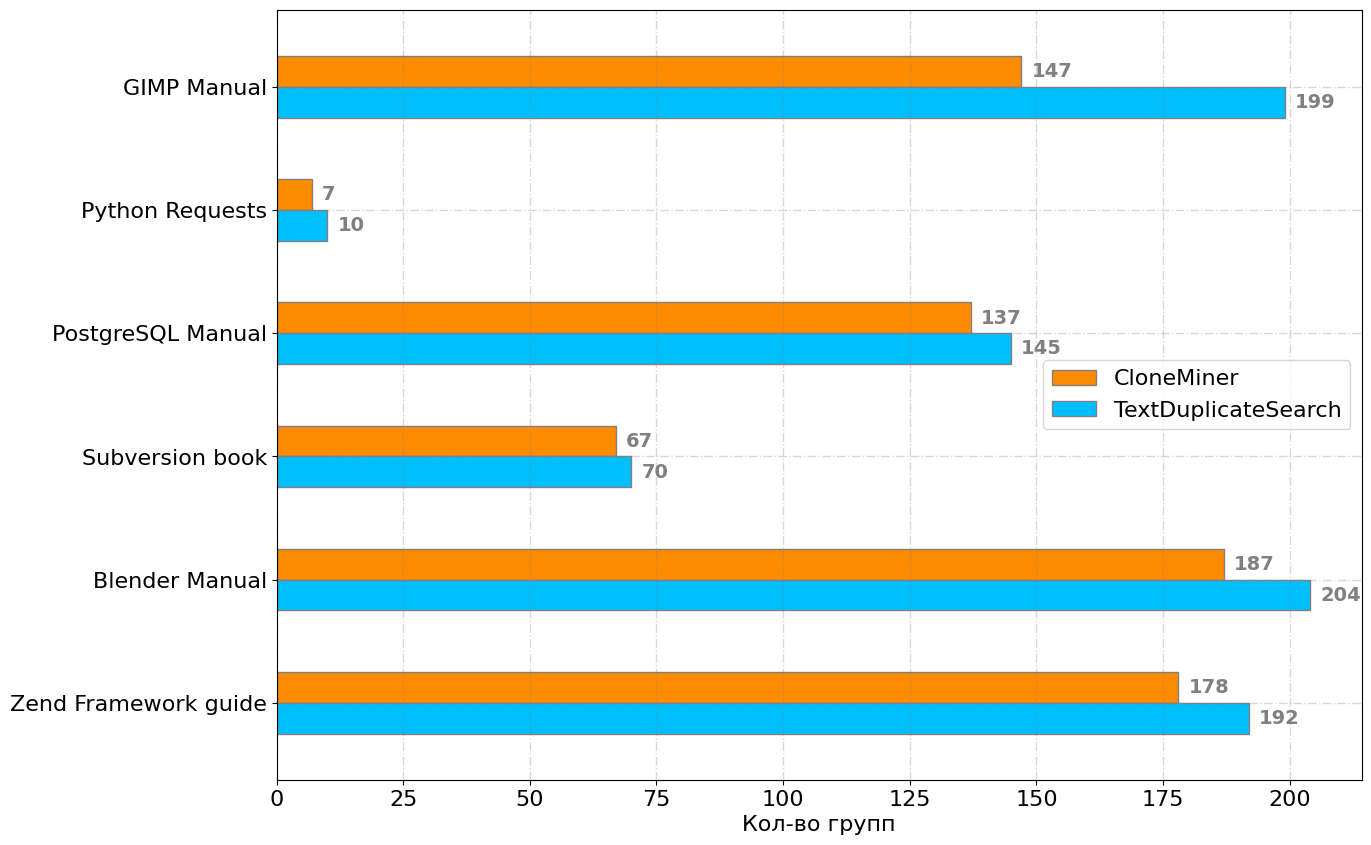
\includegraphics[scale=0.32]{../diploma/pictures/Comp2.png}
	\end{figure}
	
	\note{
		А на этом --- в результате поиска повторов с последующей обработкой DuplicateFinder'ом. Количество групп CloneMiner'а уменьшилось заметно сильнее. Это происходит потому, что CloneMiner создает много групп с пересечениями, которые отфильтровываются при обработке как незначимые.
	}
\end{frame}

%===============================================================================

\begin{frame}\frametitle{Тестирование: сравнение с CloneMiner}
	\begin{figure}[h!]
		\centering
		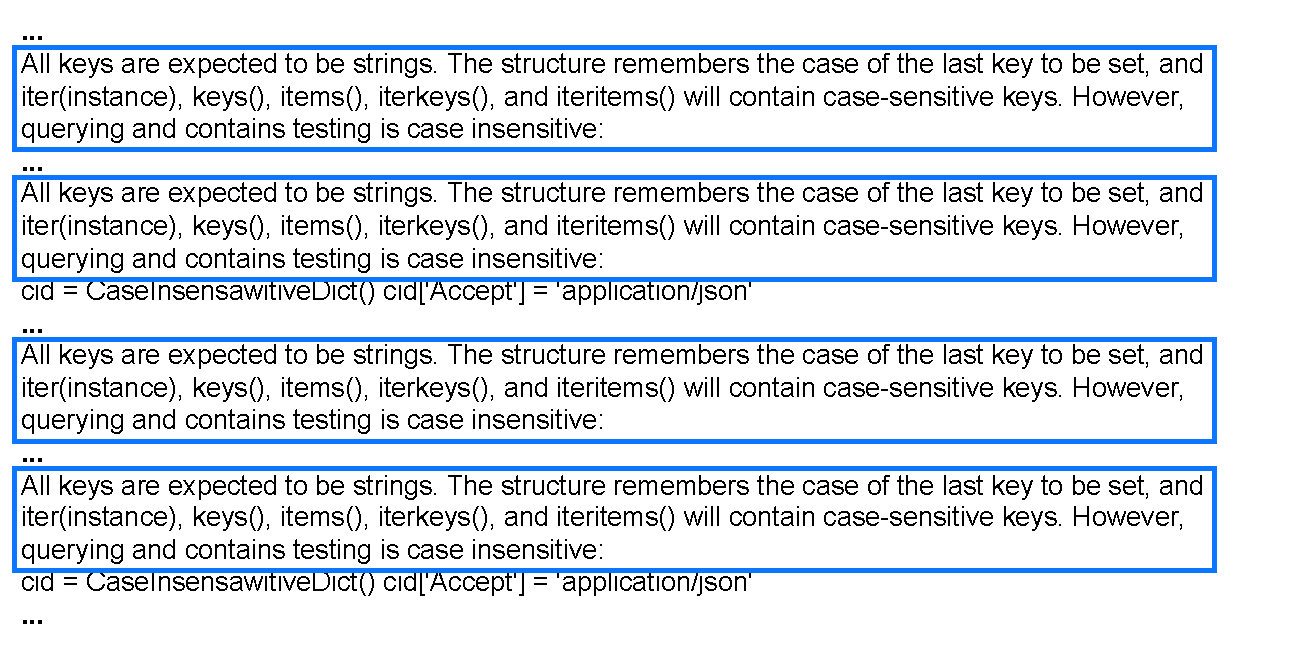
\includegraphics[scale=0.54]{pictures/Example2.pdf}
	\end{figure}
	
	\note{
		Например, в случае если есть несколько фрагментов, образующих группу повторов, при этом у некоторых из них имеются продолжения, которые совпадают, CloneMiner создаст еще одну группу не в зависимости от их размера, ...
	}
\end{frame}

%===============================================================================

\begin{frame}\frametitle{Тестирование: сравнение с CloneMiner}
	\begin{figure}[h!]
		\centering
		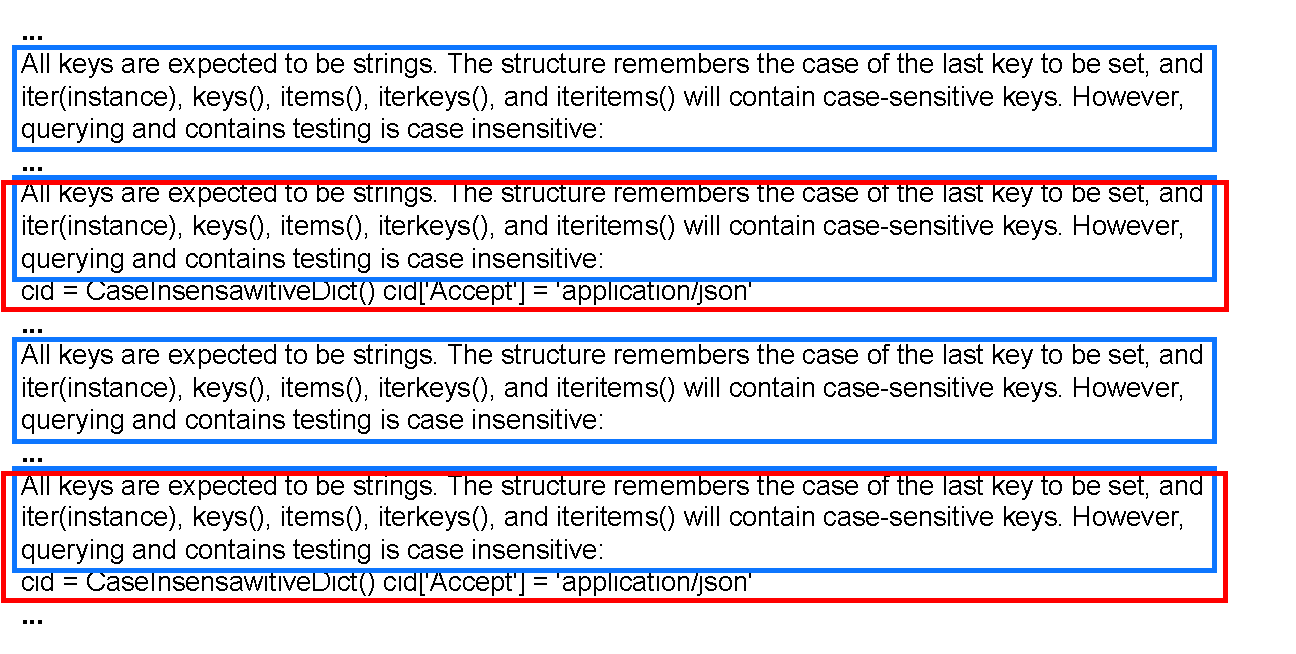
\includegraphics[scale=0.54]{pictures/Example3.pdf}
	\end{figure}
	
	\note{
		...которая затем будет отфильтрована DuplicateFinder'ом. Разработанный инструмент при этом всегда создает группы более логично и без пересечений, из-за чего результаты получаются более осмысленные и DuplicateFinder отсеивает гораздо меньше групп.
	}
\end{frame}

%===============================================================================

\begin{frame}\frametitle{Заключение}
	
	\begin{enumerate}
		\item Проанализированы основные подходы, используемые в существующих инструментах для поиска повторов
		\item Выявлены требования к новому механизму поиска
		\item Спроектирован конвейер для механизма поиска: предобработка текста, применение алгоритмов поиска повторов, балансировка групп повторов
		\item Разработаны алгоритмы для точного и неточного поиска повторов на основе использованных в Duplicate Finder инструментов
		\item Выполнена реализация инструмента на языке Python, исходный код выложен на GitHub; проведена интеграция с Duplicate Finder
		\item Проведено тестирование инструмента на корпусе документов, по результатам работы собрана статистика и проведен ее анализ
	\end{enumerate}

	\note{
		Таким образом, были достигнуты следующие результаты.
	}
\end{frame}

%===============================================================================

\end{document}